\documentclass[border=2pt]{standalone}
\usepackage{tikz}
\usetikzlibrary{automata,positioning}
\begin{document}
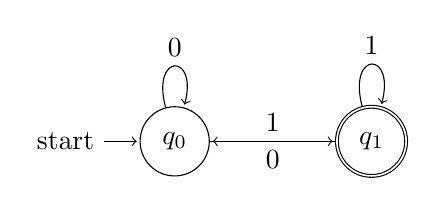
\begin{tikzpicture}[shorten >=1pt, node distance=2.5cm, auto]
  \node[state, initial] (q0) {$q_0$};
  \node[state, accepting, right of=q0] (q1) {$q_1$};
  \draw[->] (q0) to[loop above] node {0} (q0);
  \draw[->] (q0) to node {1} (q1);
  \draw[->] (q1) to[loop above] node {1} (q1);
  \draw[->] (q1) to node {0} (q0);
\end{tikzpicture}
\end{document}
